\chapter{Observations}

In this final chapter, we will discuss the performance of various ORM packages
based on the benchmarks conducted. The chapter is divided into three main
sections: Package Information, Flexibility Assessment, and Performance Test
Results.

The Package Information section provides an overview of each package, including
the supported database engines, the version used for comparison, popularity
statistics, and runtime support. This information is essential for understanding
the background and scope of each ORM package and its suitability for different
project requirements.

Next, the Flexibility Assessment section evaluates each package's adaptability
by determining whether the test was implemented using native ORM functions, the
query builder, or raw SQL with parameters. This section will also highlight any
issues or challenges encountered while working with each ORM framework.
Understanding the flexibility of each package enables developers to make
informed decisions regarding the ORM that best fits their needs and project
constraints.

Finally, the Performance Test Results section presents the outcomes of each
test, focusing on cases where query composition, operator selection, or
introduced overhead could play a measurable role in the package's performance.
These tests were conducted using the BenchmarkRunner, the frameworks connected
to a PostgreSQL instance in Docker, on an AMD Ryzen 6850U processor @ 2.7GHz,
Debian GNU/Linux 11 (bullseye) operating system, 32GB of LPDDR5-6400 RAM, and
SSD storage.

By examining the performance of each ORM package in these three areas,
developers can gain valuable insights into the advantages and limitations of
each framework, ultimately guiding them in choosing the most appropriate
solution for their projects.

\section{Package Information}

While evaluating the ORM frameworks, the latest stable branch version was used
for testing at the time of writing. It is important to note that a new version
3.0.2 of Objection.js was released after the testing was completed; however,
this update does not introduce any new features, only addressing issues with
types and ESM support.

Table \ref{table:PackageInfo} provides the exact versions used for each package,
along with the number of runtime dependencies required (excluding optional
packages and database drivers). To assess the availability and popularity of
these packages, Table \ref{table:Popularity} lists each package with popularity
metrics such as weekly downloads from the npm repository and GitHub stars given
to the project. The data was collected on the 10th of April, 2023.

\begin{table}[htb]
  \centering
  \caption{Runtime package information in test environment}
  \label{table:PackageInfo}
  \begin{tabular}{lrr}
  \hline
  \thead{Package} & \thead{Runtime dependencies} & \thead{Tested Version} \\ \hline
  PgTyped & 3 & 2.0.1 \\ 
  Zapatos & 0 & 6.1.4 \\ 
  @Databases/pg & 15 & 5.4.1 \\ 
  Objection.js & 2 & 3.0.1 \\
  MikroORM & 7 & 5.6.16 \\ 
  PrismaORM & 1 & 4.10.1 \\
  TypeORM & 14 & 0.3.12 \\ 
  Knex.js & 14 & 2.4.2 \\ 
  Sequelize & 16 & 6.31.0 \\ \hline
  \end{tabular}
\end{table}
\section{Flexibility Assessment}

The primary aspect of the comparison between individual ORM packages is their
ability to implement advanced SQL constructs using a more unified API for the
programming language. Although abstraction introduces additional logic that
requires processing power, it should offer functionality that approaches the
capabilities of direct SQL usage. A framework requiring developers to introduce
abstraction but still necessitates writing SQL queries, as the request cannot be
expressed through the API, is considered less effective as an abstraction layer
than one that can perform such requests.

Tables \ref{table:EntityTraversal}, \ref{table:SpecialSQLActions}, and
\ref{table:EdgeCases} showcase the layers used to perform the required
functionality for the benchmark. A requirement for each implementation was that
the logic had to be consistently implemented on the database, with the framework
only composing the query and parsing the result. For example, it was not allowed
to check for an existing object in an upsert operation by querying the database
independently.

\newpage

The order for implementation was as follows:
\begin{enumerate}
  \item Native methods that abstract the database logic (Native)
  \item The integrated query builder (QB)
  \item Manually written queries in SQL (SQL)
\end{enumerate}
If the operation was impossible to perform or resulted in problems, the lower
level was attempted, and the first successful one is listed in the tables.

Several notable observations can be made from the flexibility comparison.
PrismaORM stands out as the only ORM capable of natively implementing the entire
logic for each test, thanks to its unique support for increment and decrement
logic over upsert operations. The other full-fledged ORM packages in the
comparison, such as Sequelize, TypeORM, and MikroORM, performed similarly but
could not express upsert incrementation natively.

MikroORM held an advantage over TypeORM, using Knex.js as its query builder,
which could express the operation. In contrast, TypeORM's internal query builder
could not. On the other hand, Zapatos was the only package that partially failed
in any test. It could not correctly parse bigint values from PostgreSQL as
strings or BigInt primitives in JavaScript when using native methods, casting
the result into a number instead. However, this issue was resolved when a
manually written query was used.

Lastly, it is worth noting that only @databases/pg parsed bigint values into
JavaScript BigInt primitives. All other packages returned character
representations of the value. 


\begin{table}[htbp]
\centering
    \begin{threeparttable}[b]

    \caption{Entity Traversal Benchmark implementation methods}
    \label{table:EntityTraversal}
    \begin{tabular}{lccc}
    \thead{Package}    & \thead{getCatColor} & \thead{countCatsByColor} & \thead{getToysAvailableToCat} \\ \hline
    @Databases/pg & SQL\tnote{1} & SQL\tnote{1} & SQL\tnote{1} \\ 
    Knex & QB & QB & QB \\
    Kysely & QB & QB & QB \\ 
    MikroORM & Native & Native & Native \\
    Objection.js & Native & Native & Native \\ 
    PgTyped & SQL & SQL & SQL \\ 
    PrismaORM & Native & Native & Native \\ 
    Sequelize & Native & Native & Native \\ 
    TypeORM & Native & Native & Native \\ 
    Zapatos & Native & SQL\tnote{1} & SQL\tnote{1} \\ \hline
    \end{tabular}
    \begin{tablenotes}
        \item [1] With type support in template fields
      \end{tablenotes}
   \end{threeparttable}
\end{table}

\begin{table}[htbp]
\centering
    \begin{threeparttable}[b]
    \caption{Special SQL Actions Benchmark implementation methods}
    \label{table:SpecialSQLActions}
    \begin{tabular}{lccccc}
    \hline
    \thead{Package} & \thead{Upsert} & \thead{JSON \\ type} & \thead{JSON \\ Where} & \thead{Transaction} & \thead{Like \\ Query} \\ \hline
    @Databases/pg & SQL\tnote{1} & Native & Native & Native & SQL\tnote{1} \\ 
    Knex & QB\tnote{2} & QB & QB & QB & QB \\ 
    Kysely & QB\tnote{2} & QB & QB & QB & QB \\ 
    MikroORM & QB\tnote{2} & Native & Native & Native & Native \\ 
    Objection.js & QB\tnote{2} & QB & QB & Native & QB \\ 
    PgTyped & SQL & SQL & SQL & SQL & SQL \\ 
    PrismaORM & Native & Native & Native & Native & Native \\ 
    Sequelize & SQL & Native & Native\tnote{3} & Native & Native \\ 
    TypeORM & SQL & Native & Native & Native & Native \\ 
    Zapatos & Native\tnote{2} & Native & SQL\tnote{1} & Native & SQL\tnote{1} \\ \hline
    \end{tabular}
    \begin{tablenotes}
        \item [1] With type support in template fields
        \item [2] Raw SQL for increment on update
        \item [3] Raw SQL for fetching key value as promoted nested keys did not result in syntactically correct query
      \end{tablenotes}
   \end{threeparttable}
\end{table}

\begin{table}[htbp]
\centering
    \begin{threeparttable}[b]
    \caption{Edge Cases Benchmark implementation methods}
    \label{table:EdgeCases}
    \begin{tabular}{lcc}
    \hline
    \thead{Package} & \thead{SQL Injection} & \thead{BigInt handling} \\ \hline
    @Databases/pg & SQL\tnote{1} & Native\tnote{4} \\ 
    Knex & QB & QB\tnote{3} \\ 
    Kysely & QB & QB\tnote{3} \\ 
    MikroORM & Native & Native\tnote{3} \\ 
    Objection.js & QB\tnote{2} & QB\tnote{2} \tnote{,} \tnote{3} \\
    PgTyped & SQL & SQL\tnote{3} \\ 
    PrismaORM & Native & Native\tnote{3} \\
    Sequelize & Native & Native\tnote{3} \\
    TypeORM & Native & Native\tnote{3} \\ 
    Zapatos & SQL\tnote{1} & SQL\tnote{3} \tnote{,} \tnote{5} \\ \hline
    \end{tabular}
    \begin{tablenotes}
        \item [1] With type support in template fields
        \item [2] Query builder attached to model
        \item [3] Value returned as string
        \item [4] Value returned as BigInt
        \item [5] Native method converted value to Number, losing precision
      \end{tablenotes}
   \end{threeparttable}
\end{table}

\newpage
\section{Latency benchmark results}

The second aspect of the benchmarking process involved evaluating the
performance of the various packages. This evaluation focused on the optimality
of the queries formulated by each package and the overhead introduced by the
composition of the queries and result parsing. Through code analysis, the
pgTyped package was expected to exhibit minimal overhead and the most efficient
manually written queries. Consequently, pgTyped was employed as a reference for
optimal queries and minimal performance.

Several noteworthy observations emerged from the testing process. The most
apparent performance loss occurred with Objection.js during the getColorLatency
test shown in \autoref{fig:getColorLatency}. This performance loss resulted from
Objection.js favouring multiple dependent queries over a single query with joins
when utilizing the withGraphJoined method. While it would have been possible to
rewrite the query using the integrated query builder and resolve the issue, this
approach would compromise the flexibility testing and be thus considered
inadvisable.

Another fascinating result was the exceptional performance of MikroORM in the
JSONColumn test, results of which are in \autoref{fig:JSONColumn}, where it
surpassed even the pgTyped reference. This performance advantage can be
attributed to MikroORM's caching mechanism, which leverages primary keys within
its entityManager to prevent repeated database queries for the same data,
yielding faster results than the reference. This feature can be highly
beneficial for a skilled developer, but can also cause problems, if the
developer does not know about it.

Kysely demonstrated comparable capabilities to Knex while offering an enhanced
developer experience through type safety. Both Sequelize and TypeORM exhibited
similar performance levels; however, TypeORM provided superior types for methods
and filters. MikroORM, though smaller in scale, proved to be functionally rich
and benefited from access to the well-established and thoroughly tested Knex.js
query builder when model methods were insufficient.

Most ORMs lost out to query builders mainly because they prefer left joins over
stricter inner joins for many select operations. This behaviour is primarily
caused by the inability to specify precisely all the details necessary for the
realization of a query in a relational schema using the model schema these
packages used. PrismaORM avoided many of these mistakes thanks to its more
expressive and purpose-built prisma schema, which can be more expressive than
class or object definition.

Other than the few noted exceptions, the test results were as expected, with
packages using less abstraction of the database logic being able to use optimal
queries, which gave them an advantage over generic ORM queries.
Object-relational mapping packages carry a drawback of possible less optimal
data path resolution, as shown by Objection.js results in
\autoref{fig:getColorLatency} or \autoref{fig:getToysAvailableToCat}. However,
the drawback is only prominent when dealing with complex queries involving
multiple joins. It is preferable to use ORMs where the amount of data in the
database will not result in suboptimal computation time, as the overhead of the
package itself is negligible. Figures \ref{fig:countCatsByColor} and
\ref{fig:JSONColumn}, \ref{fig:JSONWhere}, \ref{fig:transactions},
\ref{fig:likeQuery} (included in the appendix) show that while the relative
performance of the queries is almost double that of reference, it is still minor
for the amount of data usually considered for most smaller projects. When
considering enterprise-level databases, the toll in which the suboptimal queries
can result will accumulate. It can result in redundant work as the application
must be repeatedly optimized while the ORM obfuscates which application
operation is causing the slowdown. 


\begin{figure}[htbp]
  \caption{getColorLatency Results}
  \label{fig:getColorLatency}
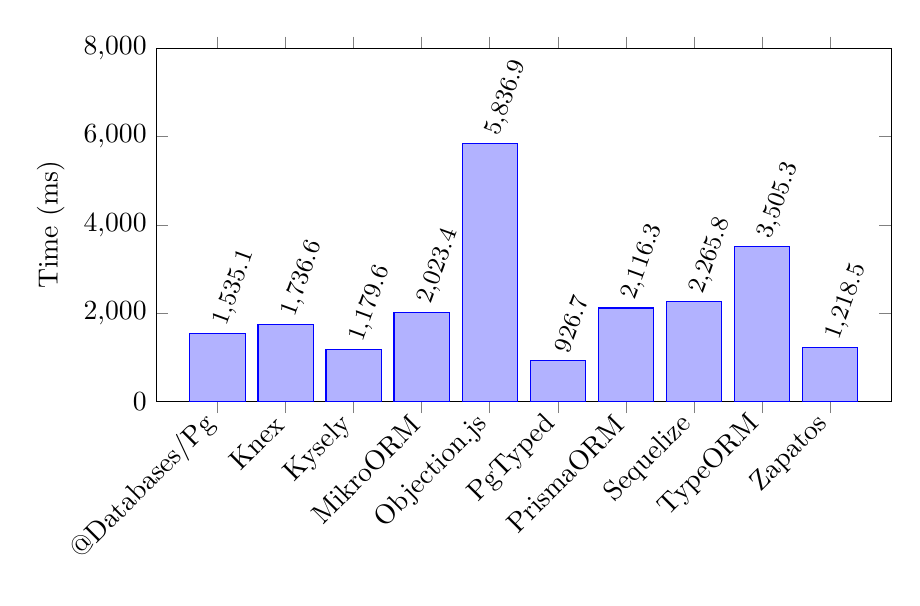
\begin{tikzpicture}
\begin{axis}[
    ybar,
    ylabel={Time (ms)},
    width=0.9\textwidth,
    height=0.5\textwidth,
    symbolic x coords={@Databases/Pg, Knex, Kysely, MikroORM, Objection.js, PgTyped, PrismaORM, Sequelize, TypeORM, Zapatos},
    xtick=data,
    xticklabel style={rotate=45, anchor=east},
    enlarge x limits=0.1,
    ybar=0.6pt,
    ymin=0,
    bar width=20pt,
    nodes near coords,
    point meta=explicit,
    ymax=8000,
    every node near coord/.append style={
        anchor=west,
        rotate=70,
        color=black,
        font=\small
    }
]
\addplot coordinates {
    (@Databases/Pg,1535.097840756178) [1535.1]
    (Knex,1736.573092713952) [1736.6]
    (Kysely,1179.5744509845972) [1179.6]
    (MikroORM,2023.4176180809736) [2023.4]
    (Objection.js,5836.859560698271) [5836.9]
    (PgTyped,926.7410168200731) [926.7]
    (PrismaORM,2116.3281450271606) [2116.3]
    (Sequelize,2265.8307730853558) [2265.8]
    (TypeORM,3505.274578973651) [3505.3]
    (Zapatos,1218.4777629077435) [1218.5]
};
\end{axis}
\end{tikzpicture}
\end{figure}

\begin{figure}[htbp]
    \caption{countCatsByColor Results}
    \label{fig:countCatsByColor}
    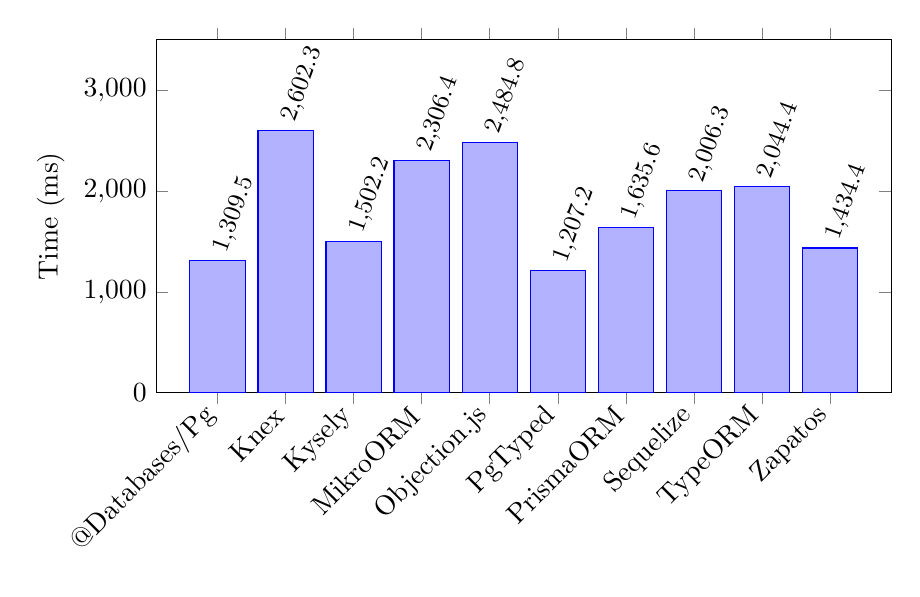
\begin{tikzpicture}
    \begin{axis}[
        ybar,
        ylabel={Time (ms)},
        width=0.9\textwidth,
        height=0.5\textwidth,
        symbolic x coords={@Databases/Pg, Knex, Kysely, MikroORM, Objection.js, PgTyped, PrismaORM, Sequelize, TypeORM, Zapatos},
        xtick=data,
        xticklabel style={rotate=45, anchor=east},
        enlarge x limits=0.1,
        ybar=0.6pt,
        ymin=0,
        bar width=20pt,
        nodes near coords,
        point meta=explicit,
        ymax=3500,
        every node near coord/.append style={
            anchor=west,
            rotate=70,
            color=black,
            font=\small
        }
    ]
    \addplot coordinates {
        (@Databases/Pg,1309.4879860281944) [1309.5]
        (Knex,2602.347664758563) [2602.3]
        (Kysely,1502.2189705818892) [1502.2]
        (MikroORM,2306.355122476816) [2306.4]
        (Objection.js,2484.835059866309) [2484.8]
        (PgTyped,1207.1816981732845) [1207.2]
        (PrismaORM,1635.5703312009573) [1635.6]
        (Sequelize,2006.3121870160103) [2006.3]
        (TypeORM,2044.3862129747868) [2044.4]
        (Zapatos,1434.3911019712687) [1434.4]
    };
    \end{axis}
    \end{tikzpicture}
\end{figure}

\begin{figure}[htbp]
  \caption{getToysAvailableToCat Results}
  \label{fig:getToysAvailableToCat}
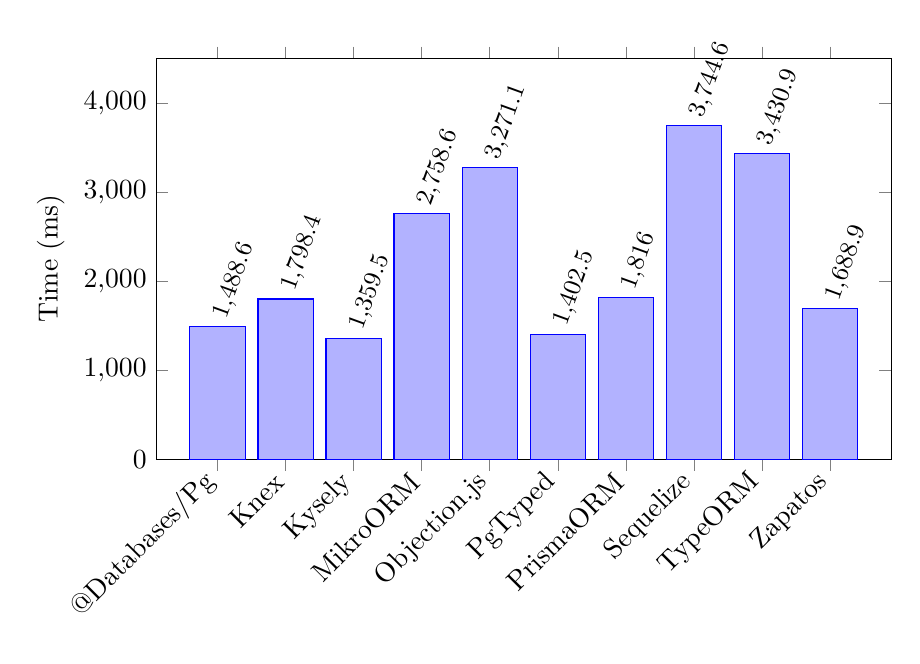
\begin{tikzpicture}
\begin{axis}[
    ybar,
    ylabel={Time (ms)},
    width=0.9\textwidth,
    height=0.55\textwidth,
    symbolic x coords={@Databases/Pg, Knex, Kysely, MikroORM, Objection.js, PgTyped, PrismaORM, Sequelize, TypeORM, Zapatos},
    xtick=data,
    xticklabel style={rotate=45, anchor=east},
    enlarge x limits=0.1,
    ybar=0.6pt,
    ymin=0,
    bar width=20pt,
    nodes near coords,
    point meta=explicit,
    ymax=4500,
    every node near coord/.append style={
        anchor=west,
        rotate=70,
        color=black,
        font=\small
    }
]
\addplot coordinates {
    (@Databases/Pg,1488.6116498708725) [1488.6]
    (Knex,1798.4078266173601) [1798.4]
    (Kysely,1359.543210029602) [1359.5]
    (MikroORM,2758.642989948392) [2758.6]
    (Objection.js,3271.0765001922846) [3271.1]
    (PgTyped,1402.466100037098) [1402.5]
    (PrismaORM,1816.036514788866) [1816.0]
    (Sequelize,3744.591591015458) [3744.6]
    (TypeORM,3430.901762366295) [3430.9]
    (Zapatos,1688.8580559790134) [1688.9]
};
\end{axis}
\end{tikzpicture}
\end{figure}

\begin{figure}[htbp]
    \caption{JSON Column handling Results}
    \label{fig:JSONColumn}
    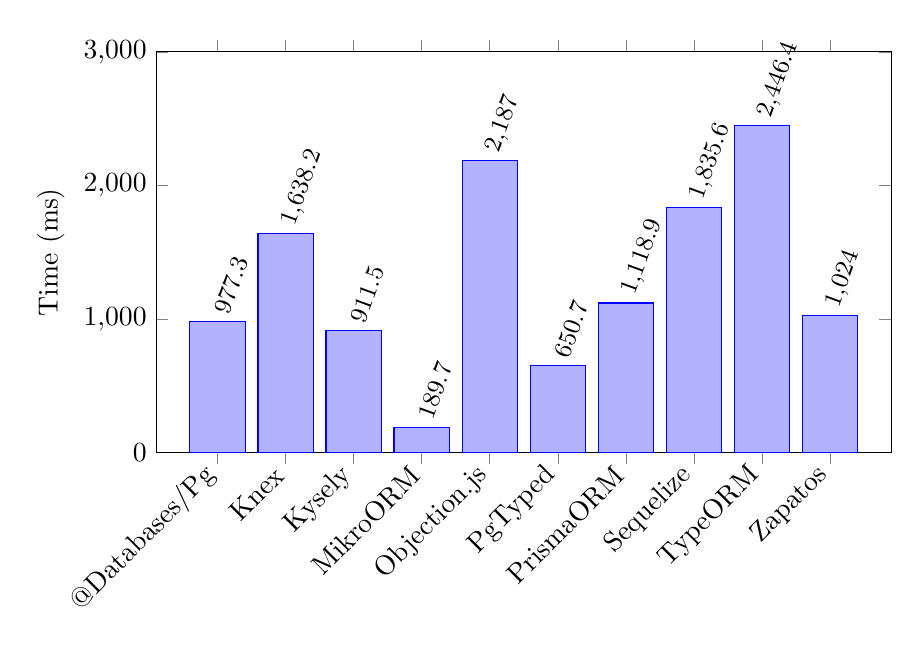
\begin{tikzpicture}
    \begin{axis}[
        ybar,
        ylabel={Time (ms)},
        width=0.9\textwidth,
        height=0.55\textwidth,
        symbolic x coords={@Databases/Pg, Knex, Kysely, MikroORM, Objection.js, PgTyped, PrismaORM, Sequelize, TypeORM, Zapatos},
        xtick=data,
        xticklabel style={rotate=45, anchor=east},
        enlarge x limits=0.1,
        ybar=0.6pt,
        ymin=0,
        bar width=20pt,
        nodes near coords,
        point meta=explicit,
        ymax=3000,
        every node near coord/.append style={
            anchor=west,
            rotate=70,
            color=black,
            font=\small
        }
    ]
    \addplot coordinates {
        (@Databases/Pg,977.3479951769114) [977.3]
        (Knex,1638.17793110013) [1638.2]
        (Kysely,911.4529178589582) [911.5]
        (MikroORM,189.65802410244942) [189.7]
        (Objection.js,2187.0198785811663) [2187.0]
        (PgTyped,650.7294137179852) [650.7]
        (PrismaORM,1118.9338391423225) [1118.9]
        (Sequelize,1835.5736832916737) [1835.6]
        (TypeORM,2446.3783992379904) [2446.4]
        (Zapatos,1024.0263592153788) [1024.0]
    };
    \end{axis}
    \end{tikzpicture}
\end{figure}